\section{Выбор гитарного усилителя}
Типичное заблуждение начинающего гитариста - думать будто бы гитарный усилитель необходим исключительно для того чтобы усиливать сигнал электрогитары. Это не так. Основная цель гитарного усилителя - в формировании звука наравне с самим инструментом. Любой, знакомый с рок-музыкой человек знает, что на свете существует множество самых разных гитарных звуков. Соответственно, они получаются на самых разных усилителях.

Фундаментальное отличие гитарного усилителя от усилителя для прослушивания музыки заключается в том, что в одном случае усилитель вносит искажения в первоначальный звуковой сигнал (гитары) ради построения нового звучания, в то время как в другом случае задача усилителя никоим образом не менять уже записанный звуковой сигнал (музыку). Таким образом эти два типа усилителя не являются взаимозаменяемыми.

Самый первый этап при выборе усилителя для любых гитарных нужд, от домашних любительских и до профессиональных концертных или студийных, это определение формата вашего будущего усилителя. Их существует несколько: “комбо”, “голова”, “рэк”, “процессор” (виртуальный усилитель). Ниже, я опишу эти форматы.

Любой гитарный усилитель состоит из трех частей, каждая из которых вносит свою долю (где-то большую, где-то меньшую) в саунд инструмента, который мы в итоге слышим.

Предусилитель, где формируется и настраивается гитарный звук.
Окончательный усилитель (он же усилитель мощности), который отвечает за регулировку громкости звука.
Специальная акустическая система (она же колонка, она же “кабинет”), через динамики которой звук “выходит в мир”. Эти колонки своею идеей также сильно отличаются от колонок для прослушивания музыки, как различаются усилители для гитары и для прослушивания музыки.
Формат “комбо” предполагает систему “все в одном корпусе”. Это наиболее популярный в мире формат гитарного усилителя.

\begin{figure}[H]
\centering
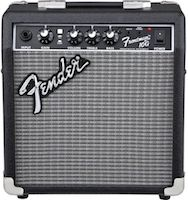
\includegraphics[width=4.5cm]{guitar-amp/guitar-amp-1.jpg}
\caption{Комбо-усилитель Fender}
\label{guitar-amp:1}
\end{figure}

Усилитель типа \textbf{“голова”} подразумевает отдельный (от колонки) аппарат (он и является “головой”), в котором находятся предусилитель и усилитель мощности. К “голове”, необходимо, подсоединять одну или несколько (зависит от модели “головы”) колонок.

\begin{figure}[h]
\centering
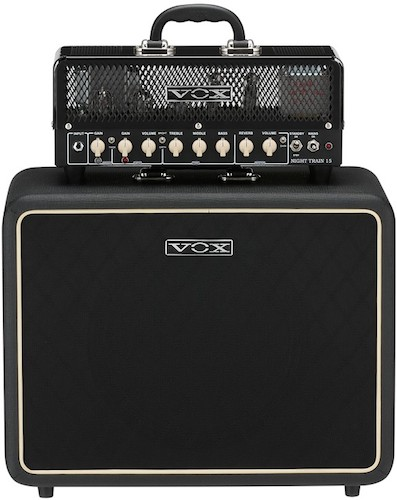
\includegraphics[width=100mm]{guitar-amp/guitar-amp-2.jpg}
\caption{Усилитель типа "голова" и кабинет VOX}
\label{guitar-amp:2}
\end{figure}

Если мы говорим о “рэке”, то речь идет о модулях, устанавливаемых в рэковые стойки. Как правило, предусилитель и усилитель мощности являются двумя самостоятельными приборами, которые соединяются между собой; могут коммутироваться с другими приборами; и, в конце концов, все это будет “уходить” в колонки.
\begin{figure}[h]
\centering
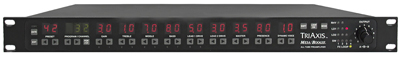
\includegraphics[width=100mm]{guitar-amp/guitar-amp-3.jpg}

\caption{Рэковый усилитель}
\label{guitar-amp:3}
\end{figure}

В настоящее время, в виде рэковых приборов могут быть не только предусилители и усилители мощности, но иногда и целые “головы”. Это делается для удобства размещения в стойке, рядом с другими приборами.

Помимо реально существующих гитарных усилителей (и их компонентов) в последние лет десять получили распространение “виртуальные усилители”. Таким термином обозначаются смоделированные методами компьютерного программирования варианты звучания как реально существующих усилителей, так и усилителей, которых никогда не существовало за пределами компьютерных программ.

Соответственно, для игры через “виртуальные усилители” используются два типа приборов: либо компьютеры c соответствующим программным обеспечением, либо процессоры. Процессоры бывают самых разных конфигураций и размеров. Однако, их суть едина - это тот же компьютер с софтом, но только помимо работы со звуком гитары этот компьютер ничего делать не умеет.
\begin{figure}[h]
\centering
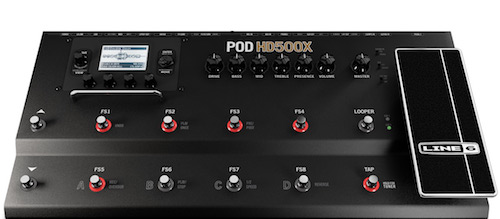
\includegraphics[width=100mm]{guitar-amp/guitar-amp-4.jpg}

\caption{POD HD-500X (моя прееелесть)}
\label{guitar-amp:POD-HD500X}
\end{figure}

В отличие от “реальных” усилителей “виртуальным” не нужны гитарные колонки, поскольку они уже смоделированы вместе со всем остальным. Поэтому гитарные процессоры (и компьютеры) можно (и нужно) подключать к аппаратуре для прослушивания музыки (колонкам и усилителям). Наиболее популярными вариантами для игры через “виртуальные усилители” являются компьютерные колонки, либо студийные мониторы. \ref{guitar-amp:POD-HD500X} % меткам можно (и нужно) давать осмысленные имена

У всех форматов гитарных усилителей существуют свои более и менее привлекательные стороны. Например, в случае с “комбо” у вас нет лишних проводов между компонентами системы. И вашему усилку требуется меньше места, что в доме, что в гастрольном транспорте, поскольку “комбо” занимает меньше пространства нежели такие же “голова” с “кабинетами”. Но зато в варианте с “головой” вы имеете возможность использовать разные “кабинеты”, что расширяет звуковую палитру и предоставляет больше вариантов звука. Еще больше вариантов предлагает “система с рэками”, где помимо колонок, можно еще и комбинировать самые разные по части звука предусилители.

Конечно, больше всего удобства и вариантов звучания, содержится в системах “виртуальных усилителей”. Однако, к настоящему моменту они еще не захватили мир полностью. Помимо поклонников, у них есть и противники. Кому-то не нравится характер звука процессоров, кто-то привык к “настоящим ручкам” регулировки, кому-то неудобно играть без “дыхания живой колонки” и т.д. Тут надо иметь в виду, что ведь буквально у всего на свете есть аргументы за и против.
\begin{figure}[h]
\centering
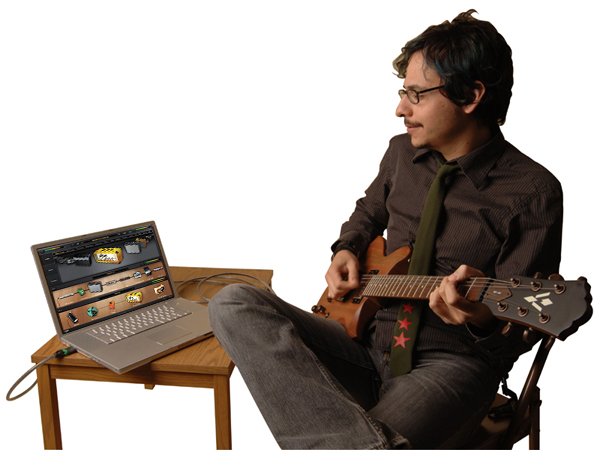
\includegraphics[width=100mm]{guitar-amp/guitar-amp-5.jpg}

\caption{Какой-то дядя с гитарой}
\label{guitar-amp:man-with-guitar}
\end{figure}

Как правило, если речь идет о профессиональных гитаристах, то у них в арсенале имеются все виды усилителей. В студии они, допустим, работают с “рэками”, на концерты возят “головы”, дома и на репетиционных базах у них могут быть \textbf{“комбо”}, а в нотбуках стоять “виртуальные”, с которыми они “балуются” в отелях во время гастрольных туров.

Если же говорить домашних усилителях обычных гитаристов-любителей, то обычно большинству хватает одного обычного “комбо”, плюс набор “виртуальных” для разного рода экспериментов. Хотя, конечно, степень увлечения гитарой бывает весьма разных масштабов. Поэтому в каждом городе можно найти множество жилищ, забитых оборудованием так, что некоторые профессиональные студии позавидуют. Тут уж у каждого человека свое представление о потребностях.

Для тех, кто только начинает свой путь в мир гитары я бы рекомендовал купить недорогой комбо. Например, Marshall MG10CF. Реальный усилитель любому будет полезен для того, чтобы поставить правильное звукоизвлечение и вообще понять (и прочувствовать) природу гитарного звука.